\documentclass[11pt,twoside,a4paper]{article}
\usepackage[english]{babel} %English hyphenation
\usepackage{amsmath} %Mathematical stuff
\usepackage{amsthm}
\usepackage{amssymb}
\usepackage{graphicx}
\usepackage{float}
\graphicspath{ {images/} }

%Hyperreferences in the document. (e.g. \ref is clickable)
\usepackage{hyperref}

%Pseudocode
\usepackage[noend]{algpseudocode}

\usepackage{a4wide,times}
\title{Emergent Architecture Design}
\author{
  Multimedia Services Team goto fail;\\
  Alex Geenen 4210891\\
  Bart de Jonge 4392256\\
  Mark van der Ruit 4228723\\
  Martijn Janssen 4316709\\
  Menno Oudshoorn 4395751
}
\begin{document}
\maketitle
\clearpage

\tableofcontents
\clearpage

\section{Introduction} \label{sec:intro}
This document provides an overview of the software system that will be built during the Multimedia Services Context Project. The architecture of this system is explored by breaking it down into its subsystems, which as a whole, come together to form a solid software package. 

\subsection{Design Goals}
Chief among the priorities within this project are the design goals:

\subsubsection{Availability}
The system will be built using an Agile process, and will utilize continuous integration to ensure that the software will always work. As such, the goal is to have a working product at the end of each development sprint, ready for use \& testing by the client. This "always ready" design encourages the completion of features within sprints, giving clear milestones, and contributes to the overall health of the project. In addition, it allows the client to give feedback after every iteration, enabling changes to be made without increasing technical debt.

\subsubsection{Modularity}
In a digital audiovisual workflow there are many different users involved, each of whom have varying software needs. In order to meet all of them, the software system has to be flexible. This flexibility is best reflected in a modular architecture, as modularity encourages code and component reuse, which in turn increases the team's efficiency (and is also a software development best practice). Instead of designing and building three or four standalone systems, this principle allows the creation a blended system which facilitates a uniform workflow (i.e. one uniform data format/protocol throughout the workflow, be it in the form of XML or otherwise). In addition, changes can be made without fear of complex interdependencies.

\clearpage % Helps figure formatting

\section{Software Architecture Views}
This section explains the architecture of the system. The overarching idea is that a program is used to plan the camera script, at which point it is uploaded to a webserver. The webserver can then be used to add camera presets, after which it can send commands to the remote IP cameras.
\subsection{Subsystem decomposition}
% Sketch of MVC
\begin{figure}[H]
	\centering
	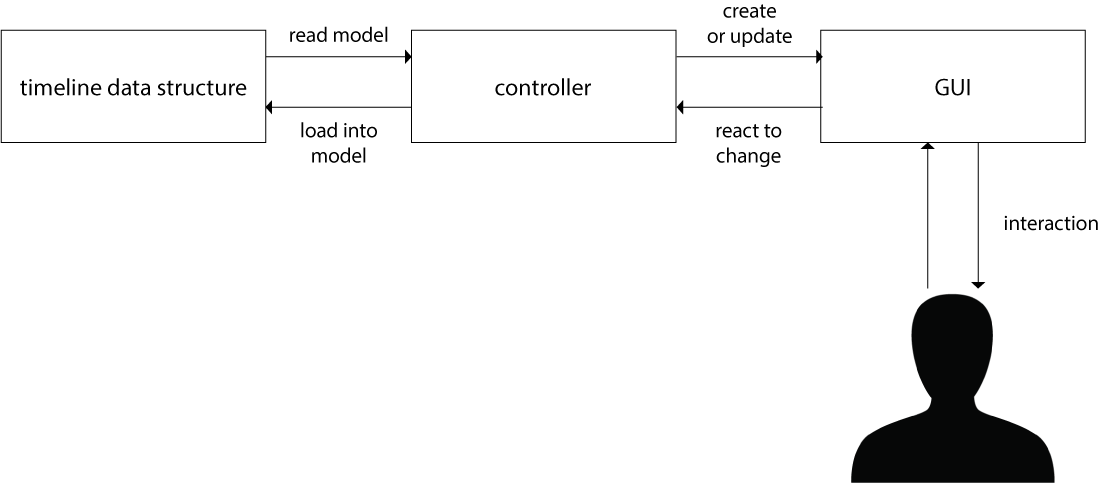
\includegraphics[width=\textwidth]{architecture-decomposition}
	\caption{Scripting Architecture}
	\label{fig:archdecomp}
\end{figure}

The architecture of the scripting software is divided up according to the Model View Controller design pattern. This pattern consists of a clear division of labor between the data model, the view that the user sees and interacts with, and the controller which ensures that the view reflects the model and vice versa.
\begin{itemize}
    \item The model: The model consists of a data structure that reflects the state of timeline for the scripting view. The timeline data encompasses the shots both for the director's script and the individual cameras.
    \item The view: The view consists of a GUI which displays the current state of the script in a timeline format, and the buttons required to add or make changes to shots and otherwise manipulate the entire script
    \item The controllers: The controller reacts to changes in the view (e.g. resizing a shot), which then trigger logic that keep the model up to date (e.g. Making sure that the shot length is updated). These adjustments are not just one way. Based on actions in the view, other portions of the view may also change, allowing complex and powerful actions to be simplified. The controller is also responsible for initializing the part of the software that it "owns". This means that it is able to load persistent data into the model, and then subsequently create the corresponding view.
\end{itemize}
The controllers have been split into two subgroups: those which create the gui, and those which are more concerned with the proper manipulation of the model. This allows a clearer separation and fine tuning of which responsiblities belong where in the project structure.\\
\begin{figure}[H]
	\centering
	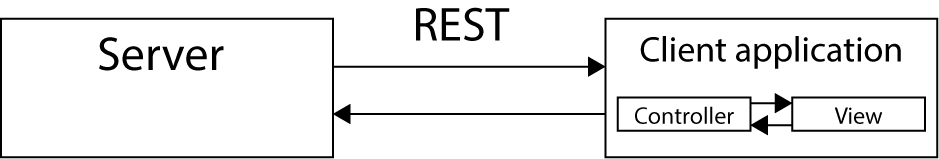
\includegraphics[width=\textwidth]{server-decomposition}
	\caption{Server Architecture}
	\label{fig:archdecomp}
\end{figure}
In addition to the scripting software, a webserver has been created which follows the REST (Representational State Transfer) architecture. This means that the server works with standard HTTP methods such as GET and POST, and that it doesn't store client session data. The session data is stored in a client's browser and, per request, the necessary session data is sent to the server in order to successfully complete the request. As the webserver is RESTful, it also operates using a clear separation of concerns between the server and the client-side application, e.g. that the server is not responsible for managing the client interface or state, and that the client is not responsible for the storage of data on the server. The client application takes the data provided by the RESTful routes and manipulates it in a View-Controller manner.

\subsection{Hardware/Software Mapping}
% Laptop to IP cameras
\begin{figure}[H]
	\centering
	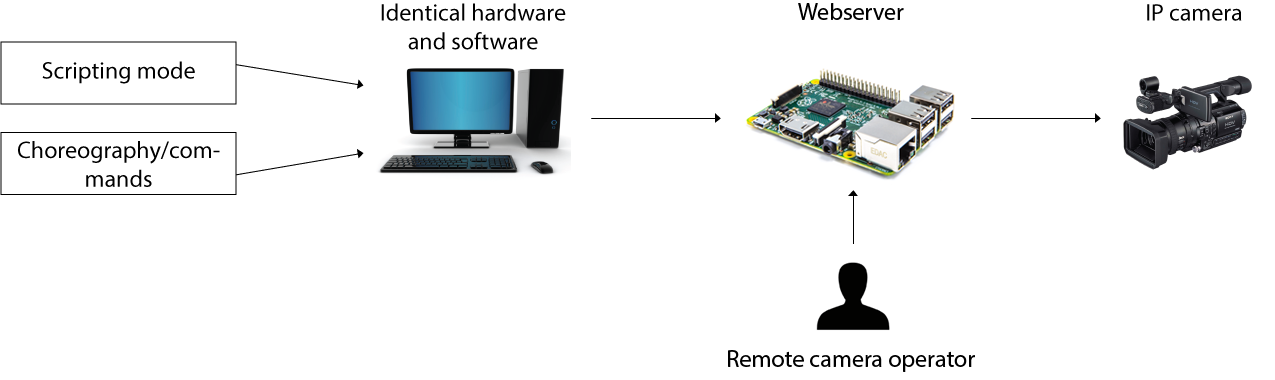
\includegraphics[width=\textwidth]{HWsoftwaremapping}
	\caption{Hardware to Software Mapping}
	\label{fig:mapping}
\end{figure}

The software for creating the director script will be used by the director. Once he/she is satisfied with the script, it can then be uploaded to a web server. At this point the remote camera operators can login to view the script, and then add camera choreography presets. In addition, the remote camera operators will be able to determine which commands will be sent to the IP cameras. When a recording is taking place the webserver will send these recorded commands to the IP cameras. If a camera operator needs to make adjustments to a shot, the webserver will yield to manual operation. The shot caller (responsible for the live timing) can also use the webserver to advance the script during live recordings.
%The hardware and software will be the same for both the director and the camera operator. The functionality of the software will differ through the use of different modes. There is one mode for the scripting, and one for camera choreography and coordination of the commands which will be sent to the IP cameras. When a recording is taking place the software will send commands from the computer to the proper cameras. The current plan is to use a server (possibly using the command design pattern) to push these commands to the IP cameras, which will allow the remote camera operators to take over whenever they deem it necessary to make changes and/or corrections.

\subsection{Persistent Data Management}
Data persistence in the system is accomplished through the use of XML files. Each script is loaded in and saved as an XML file, recording information about the timeline which can then be used by the controller to restore the program state. It also facilitates the transfer of a project between computers if necessary (e.g. from the director's computer to the camera operator's computer).

\section{Glossary}
\begin{itemize}
  \item GUI - A graphical user interface. What the user interacts with.
\end{itemize}

\end{document}
